\section{State of the Art}
\label{SoA}
%The state of the art shows that the research questions or research hypotheses are not finally answered. For this, previous works are analyzed and the gap, i.e. the difference between research questions / hypotheses and previous papers, is outlined. For this, a sufficient number of previous works are referenced. It is important to note that it is not a problem if previous works on the publication’s topic are found. If no previous works are found, maybe the research topic is simply not relevant. A gap exists as long as the research questions or research hypotheses are not finally answered, i.e. no standardized, commonly-accepted solutions exist. The state of the art section should identify structures in the state of the art. I.e. it should not only be a listing of several previous publications. Instead structures in the state of the art such as classes of similar research solutions, important research groups or important trends should be described. Referenced publications should come from Aconferences or good journals and should not be older than 3-4 year. Exceptions are seminal works, i.e. publications which are the top publications in a specific field.
\begin{figure*}[ht]
    \centering
    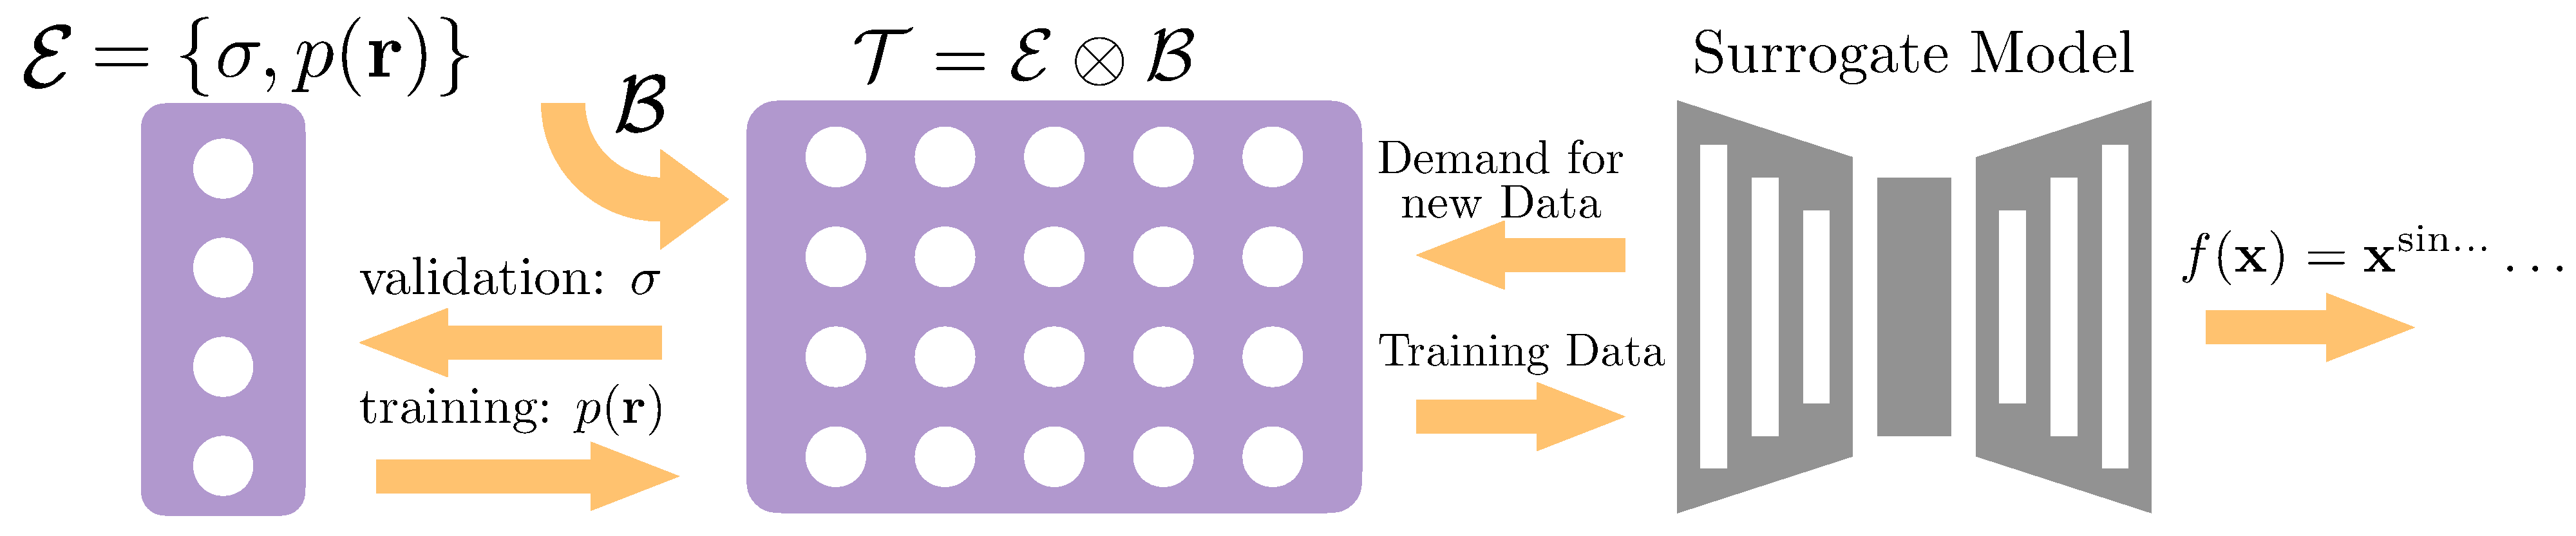
\includegraphics[width=0.95\textwidth]{images/Active_Learning.pdf}
    {\caption{\small Tiered strategy to learn materials laws; a targeted experimental program will generate realistic morphologies $\bf r$ and reference data $\sigma$. Direct physical modeling merges experimental data ${\cal E}$ with bulk data ${\cal B}$ from databases to generate large scale feature-property data ${\cal T}$. This is then used to learn a surrogate model in form of a Bayesian generative neural network autoencoder. This autoencoder can both in an active learning sense request new data points. But it can also be a basis for the generation of a symbol model, e.g. using algorithms from the field of explainable AI.}\label{fig:workflow}}%
\end{figure*}
The author group traditionally works on the edge between computer science and automation technology. Focus are ML and artificial intelligence methods for cyber-physical systems including RepL \cite{Niggemao3, Niggemao4}. 
Considering a-priori knowledge to improve ML is one big research topic. Therefore, technical systems are characterized by the abundance of a-priori knowledge such as system structures and physical laws. As a result, methods of machine learning require less data and become extrapolable. Furthermore, causal relationships are used to calculate optimizations \cite{Niggemao6, Niggemao1, Niggemao2}. These partly subsymbolic representations are used to abstract logical symbols from the physical systems \cite{Niggemao8}. %This enables the explicit representation of knowledge in interpretable formulas. Furthermore, complementary approaches are implemented to directly extract physically meaningful representations (\ldots) %\cite{Niggemao5} 
to generate surrogate models \cite{Niggemao7}.

For several years now we have been abstracting these skills into the sub-area of computational materials design or -- from an algorithmic perspective -- spatial neural networks. Often neural networks are used to analyze materials, e.g. to identify characteristics \cite{Jung-Niggemann,grossmann:2022h}.

This also includes the use of surrogate models to replace slow solver-based simulations when designing new materials \cite{rensmeyer:2023a}
 with generative and probabilistic neural networks \cite{Niggemann:2023b}.

\subsection{Physics Based Machine Learning}
The ideal physical behavior of materials can often be approximated using well-known partial differential equations (PDEs). However, the numerical solution of these equations is computationally intensive for high temporal and spatial resolutions. In addition, classic deep learning approaches fail due to a lack of labeled data. Physics-informed neural networks (PINNs) solve this contradiction \cite{Cai.2021, BPINN, PINNFlow}.

These models learn the unknown parameters in an otherwise known (partial) differential equation. To do this, the neural network is trained to interpolate between the known data points in a way that corresponds to the known form of the equation. The unknown parameters of the equation are treated as neural network parameters and optimized by gradient descent alongside the actual neural network parameters \cite{RAISSI}.

%Since they express the individual components of the PDEs in the output layers, they use only space and time coordinates as input. As a result, they lack the ability to process solutions that are already potentially given and, based on this, to elaborate representative forms of data.

%An extension of these methods for location-dependant PDEs are e.g. Physics Enhanced Convolutional Neural Networks methods \cite{PIM}. They make use of the fact that Convolutional Neural Networks are capable of effectively extracting spatial features in the data, which are then padded with the boundary conditions from the PDE. The loss function is set up in parallel as with PINNs.
An alternative to PINNs for settings where the governing equations are not already partially known is offered by an uncertainty-based active learning strategy. They have established themselves as an extremely valuable approach in areas where labeling data requires significant effort \cite{DAL}. These methods have proven capable of substantially reducing the amount of required data to train a neural network model, by only labeling data on which the model still has a high degree of uncertainty \cite{active}. Additionally, this approach makes the resulting model more robust to outliers, as exploiting uncertainty in the labeling process can be used to bias the dataset toward outlier configurations \cite{UAviaAL}. 
%For these reasons we expect active learning as well as physics enhanced models to play a significant role in the creation of substitutional models for the physical behaviour of CT based digitalized materials.

\subsection{Generative Systems Modelling}
An alternative for the spatial system description, taking complex (boundary) conditions into account, are generative AI approaches such as GANs or DDPMs. CTs help here as training data to create realistic morphologies. %\cite{loey2020deep, Jiang2020COVID19CI, mann2021generation, Peng2023CBCTBasedSC}.
% GAN for image generation

For example, GANs are used to generate a large number of CT images that have similar properties to the training images \cite{su2022microstructure}. 
In other approaches, the corresponding three-dimensional (3D) structure is derived from two-dimensional (2D) images \cite{FENG2020113043,ZHANG2021110018}.
\citet{Henkes_2022} proposes an extended method that uses a Wasserstein loss \cite{arjovsky2017wasserstein} to generate 3D microstructures with the same properties as the original data. 

However, to create morphologies with defined and changing properties, conditions-based approaches must be considered. Although there are already some approaches from the field of medical technology \cite{Jiang2020COVID19CI,Peng2023CBCTBasedSC,CganMed1} and materials design \cite{DURETH2023105608,janssens2020computed}, the underlying conditions are not multimodal or high-dimensional.

% Feature extracting
Feature engineering methods help with subsequent automated CT segmentation or classification, as well as design evaluation \cite{damewood2023representations}. Convolutional Neural Networks (CNNs) are used successfully here \cite{GOBERT2020101460,ziabari2023enabling}. However, a disadvantage of this approach is the poor interpretability of the learned features.

% Inverse materials design
The aim of these intermediate steps is a closed ML framework that covers the entire materials design process \cite{10.3389/fmats.2022.818535,pei2021machine}. The list of the previous approaches shows the possibility for abstract and idealized descriptions of materials behavior. However, since only the idealized materials behavior is described there, uncertainties regarding production and composition are not taken into account. Furthermore, explicit, interpretable, or formula-based substitution models are missing.

\subsection{Systems Representation}
RepL is the process of automatically discovering and extracting meaningful patterns and features from raw data, enabling more effective and efficient machine learning models. Autoencoders and variational autoencoders \cite{kingma:2014a} have become highly utilized methods for the extraction of physically meaningful representations of a systems observations. Nautrup et al. and Iten et al. \cite{PhysRevLett.124.010508, Nautrup} use these methods to identify the relevant variables of a physical system that are necessary for downstream computations and representation in a simple and interpretable way. Variational autoencoders have also been used to improve the interpretability of latent variables by producing discrete encodings of observations \cite{MixReps, SOMVAE, VQVAE}. The learning of discrete representations has been one of the main focuses of RepL and could potentially be used to identify different modes of behavior of materials properties. 

Champion et al. \cite{AutoSR} use an autoencoder to map the observation of the physical system to a suitable representation.  A symbolic regression of the extracted features is then performed. The symbolic form describes the desired properties of a physical system and have varying degrees of complexity depending on the chosen basis. In doing so, they describe the transition into the field of system identification. The algorithmic formulas are derived from observed data to model the behavior of dynamic systems.